
%!TEX root=../main.tex
\section{Background} 
\label{chap:background}
%todo put everything down a level
%\section{Trajectory prediction in maritime/AIS}%core SOTA werde das zusammenfassen mit related work am ende des kapitels?
\me{rename this to related work, maybe as part of introduction, tell the story leading up to my problem statement. some of this is already methodology. copy it there. also makes it more compact. problem statement and research gap after this.}
\ws{The chapter should be named related work. You can write the `Background' in the methods section}
\section{Kinematic Models} 
\ws{Please avoid stacked headings. There should be some text after the heading. Otherwise, it is better to use paragraphs rather than sections}
    \subsection{CV}
    Despite not being the state-of-the-art, the \acf{CV}-model \ws{The acronym should be introduced in full for the first time. Use `gls' for that} is still applied in vessel motion tracking  \parencite{8693856CV}. A vessel's position is predicted using the velocity (\ac{SOG}) of the last known timestamp using the assumption the vessel does not change \ac{SOG} nor \ac{COG} with in the prediction horizon. Thus, without feedback the model always generates a straight line.
    \subsection{CTRV}
    The \acf{CTRV} model relaxes the assumption of a strictly linear path. It still assumes that the \ac{SOG} remains constant throughout the prediction horizon, but it allows the course over ground \ac{COG} to change at a constant \acf{ROT}, denoted $\dot{\psi}$. Because it accounts for the vessel's rotational movement, the \ac{CTRV} model generates a circular arc rather than a straight line. This makes it  more accurate than the \ac{CV} model when predicting the trajectory of a vessel executing a turning maneuver.
    %unterschied: cog nicht konstant, sondern sog (cog_dot)
    

\section{Stochastic Filters} 
Unlike purely kinematic models, which propagate a single deterministic state estimate, stochastic filters explicitly represent uncertainty by tracking both a state estimate and a measure of confidence in that estimate.

\subsection{Kalman Filter}
\label{subsec:kalmanfilterbackground}
The Kalman Filter, first introduced by \textcite{Kalman1960}, combines model information and measurements to derive optimal filtering and to estimate the state of a dynamic system. Additionally, it contains information regarding the certainty of the estimation. \cite{ValleryDoerschel2025RTSkript} describe it as a highly efficient algorithm frequently used in applications such as navigation solutions or tracking procedures. The core operation of the Kalman Filter, as described in their lecture notes, can be summarized as a recurring two-step algorithm of prediction and correction:
\begin{itemize}
    \item \textbf{Prediction}: The filter executes a pure forward simulation based on the system model and the previously estimated state. This step provides the best possible prediction of the state for the upcoming time step.
    \item \textbf{Correction}: When a measurement becomes available, the algorithm determines the deviation between the actual measured signal and the predicted output. The filter then corrects the prediction based on this deviation. This correction step functions as a least-square problem, utilizing weighting matrices to determine whether the filter should trust the model prediction or the sensor measurement more.
\end{itemize}
The fundamental Kalman Filter assumes a linear system and linear measurement equations, and it is the optimal estimator for linear systems with gaussian noise.


\subsection{Extended Kalman Filter}

For non-linear systems, this filter can be extended. The Extended Kalman Filter \parencite{Schmidt1966EKF} addresses the limitations of the standard approach by locally linearizing the non-linear system equations around the most recent state estimates. Specifically, the state transition model is linearized around the previously corrected state, while the measurement function is linearized around the newly predicted state. While the pure forward simulation of the state itself is executed using the actual non-linear model, the filter uses these local linearizations to update the covariances and to compute the correction step. This approach allows the EKF to treat non-linear systems consistently within the structure of the standard Kalman Filter \parencite[445]{ValleryDoerschel2025RTSkript}.


\section{Sequence-to-Sequence Models}   
    %https://arxiv.org/html/2406.02770v1#bib.bib14


    In the domain of Deep Learning, \ac{S2S}  Models serve as a framework for tasks where input and output are dependent sequences. While \ac{S2S} is rooted in language processing tasks like translation \cite{sutskever2014sequencesequencelearningneural}, it can be %dieses zitat vlt raus
    applied to any kind of sequential data, ranging from numerical time series and sensor data to genomes and handwriting \cite{gentleschmidt2019recurrentneuralnetworksrnns}. 
    Most \ac{S2S} models follow an \textbf{Encoder-Decoder} architecture. 
    \begin{itemize}
        \item \textbf{Encoder}: Processes the input sequence and compresses the information into a fixed-size context vector (hidden state).
        \item \textbf{Decoder}: Uses this vector to generate the output sequence (e.g., the predicted GPS positions for the next 10 time steps).
    \end{itemize}
    A graphical overview of Encoder Decoder Sequence Models using the following buidling blocks can be found in Figures \ref{fig:s2s_rnn_appendix}, \ref{fig:s2s_lstm_appendix}, \ref{fig:s2s_bilstm_appendix}, and \ref{fig:s2s_attention_appendix}:

    %Encoder and Decoder can for example be built with the following two building blocks:%bessere überleitung todo

    \subsection{RNN}
    Building on the first popular model to use recurrence, the Hopfield Network introduced by \cite{hopfieldrnn}, the foundational concept for sequence-based learning is the \ac{RNN}. 
    The primary distinction between \acp{RNN} and conventional Feedforward Neural Networks, such as \acp{MLP}, is the direction of information flow. While Feedforward Networks are acyclic, \acp{RNN} use cycles to feed information back into the hidden state, the \textit{memory}. This architecture allows the model to incorporate historical context from previous inputs $X_{0:t-1}$ when processing the current input $X_t$, rather than treating each input in isolation \cite{gentleschmidt2019recurrentneuralnetworksrnns} and to make decisions based on the patterns it recognizes \cite{AIBook}. The recurrence can be expressed as:

    \begin{equation}
        H_t = \phi_h (X_t W_{xh} + H_{t-1} W_{hh} + b_h) % liefert eigentlich keinen mehrwert
    \end{equation}
    where $W$ represents weight matrices and $\phi$ an activation function. Despite their theoretical capability to handle sequences, \acp{RNN} suffer from the \textit{vanishing gradient problem}, as well as the \textit{exploding gradient problem}, as has been established by \cite{279181bengio}. As the sequence length increases, the gradients used to update weights during backpropagation decrease exponentially, preventing the model from learning long-term dependencies.
    %wenn gefragt, für eine kurze definition der PRobleme, \cite{AIBook}
    
    \subsection{LSTM}
     To address the limitations of standard \acp{RNN} in capturing long-term dependencies, \cite{hochreiterLSTM} introduced the \ac{LSTM} architecture. The core innovation of the \ac{LSTM} is the introduction of a cell state $C_t$, which allows information to persist across many time steps. The flow of information in and out of these cells is regulated by three \textbf{gates}: The
    \begin{itemize}
        \item \textbf{Forget Gate $F_t$}:  Determines which information from the previous cell state $C_{t-1}$ is no longer needed and should be discarded.
        \item \textbf{Input Gate $I_t$}: Decides which new information from the current input $X_t$ and previous hidden state $H_{t-1}$ is relevant to be stored in the cell state.
        \item \textbf{Output Gate $O_t$}: Controls which parts of the current cell state $C_t$ are used to compute the new hidden state $H_t$.
    \end{itemize}
    
     Following the formalization by \cite{gentleschmidt2019recurrentneuralnetworksrnns}, the internal update process is defined by the following set of equations:
     \begin{align}
         F_t &= \sigma(X_t W_{xf} + H_{t-1} W_{hf} + b_f) \\%forget
         I_t &= \sigma(X_t W_{xi} + H_{t-1} W_{hi} + b_i) \\%input
         \tilde{C}_t &= \tanh(X_t W_{xc} + H_{t-1} W_{hc} + b_c) \\%input candidate
         C_t &= F_t \odot C_{t-1} + I_t \odot \tilde{C}t \\ % update by multiplying old with forget and adding new
         O_t &= \sigma(X_t W{xo} + H_{t-1} W_{ho} + b_o) \\ %output: which part of memory is relevant?
         H_t &= O_t \odot \tanh(C_t)
     \end{align}
     
     In these equations, $\tilde{C}_t$ represents a candidate cell state, $\sigma$ is the sigmoid activation function $\sigma(x) = \frac{1}{1 + e^{-x}}$, and $\odot$ denotes the element-wise (Hadamard) product. By using an this update for the cell state $C_t$, the \ac{LSTM} prevents the gradient from vanishing as quickly as in standard \acp{RNN}, allowing the network to learn relationships across significantly larger time gaps.

     As indicated by the multi-dimensional input vector $X_t$ and the associated weight matrices, the \ac{LSTM} architecture is mathematically equipped for multivariate sequence modeling. The model has the capacity to represent nonlinear cross-channel correlations, because the internal gating mechanisms integrate information from all input features simultaneously to model their interdependencies within a shared hidden representation, making it suitable for our usecase. 
     %achtung (für methodik:) LSTM erwarten gleichbleibende frequenz, informationsverlust durch interpolieren
    

    \subsubsection{Bi-LSTM}
    Many variants and extensions of the \ac{LSTM} have been proposed to enhance its representative power. A notable architectural advancement is the \ac{Bi-LSTM}. While \cite{sutskever2014sequencesequencelearningneural} demonstrated that simply reversing the input sequence in a unidirectional \ac{S2S} model can significantly improve performance, the \ac{Bi-LSTM}, first introduced by \cite{articlebilstmorigins} formalizes this concept in its architecture .
    
    A \ac{Bi-LSTM} consists of two parallel hidden layers: a \textit{forward \ac{LSTM}} that processes the sequence in chronological order and a \textit{backward \ac{LSTM}} that processes it in reverse. Their respective hidden state outputs are then concatenated, added, averaged or multiplied  to form the final output. 
    Recent studies, such as \cite{articlebilstmsus} claim this makes the \ac{Bi-LSTM} more suitable for vessel trajectory prediction. 
   
    However, the application of \acp{Bi-LSTM} in autonomous systems and \ac{MTT} requires us to consider causality. Because the backward pass requires knowledge of the entire sequence up to the final time step, \acp{Bi-LSTM} are non-causal. Consequently, they cannot be used within the decoder of our \ac{S2S} Model. Nevertheless, they can be applied within the encoder stage. This allows the model to generate a richer input vector, which is then processed by a unidirectional decoder to predict future motion. %blabla als  hyperparameter in optimierer.. evtl auch schon hier den teil in methologie schreiben, mit tim klörne

      % 7 zusammenfassung: xlstm besser skalierbar, größerer speicher. aber für unsere 10 timesteps overkill. außerdem größerer feature space, schwerer (Schnell) manuell zu tunen, was unsere vorteile wettmachen würde + mangelnde vergeichbarkeit weil neu, . also nur kurz erklären
    %xlstm liefert die grundlage für ein lstm basiertes foundation modell durch erweiterung mit ..., aber dieses exisistiert leider noch nicht. wenn ich den platz habe würde ich gerne

    \subsubsection{x-LSTM} \me{only really important to motivate tirex. maybe too detailed here}

    Recently, \cite{beck2024xlstmextendedlongshortterm} introduced the \ac{x-LSTM} architecture to address bottlenecks of \ac{LSTM}. The primary goals of this architecture are to improve hardware scalability and to provide a larger memory capacity. To achieve this, two new \ac{LSTM} Layers are introduced:
    
    \begin{itemize}
        \item \textbf{\ac{s-LSTM}}: introduces exponential gating, which allows the model to revise and update its memory more dynamically.
        \item \textbf{\ac{m-LSTM}}: replaces the traditional vector cell state and its element-wise updates with a matrix memory updated via matrix multiplication. This structural shift eliminates the sequential dependency of the hidden state, enabling fully parallelized sequence processing during training.
    \end{itemize}
    Using these layers, an \ac{x-LSTM} can maintain the linear time complexity $\mathcal{O}(N)$ of conventional \acp{RNN} during inference, in contrast to the quadratic complexity of Transformers. \cite{beck2024xlstmextendedlongshortterm, attentioniayn} %for respective Time omplexity 
    
    However, the application of \ac{x-LSTM} in this work introduces practical challenges. For our specific use case of predicting short 10-step trajectories, the expanded memory capacity offers limited benefits while introducing computational overhead. Further, the architecture requires additional hyperparameters, such as the choice between \ac{s-LSTM} and \ac{m-LSTM} layers, as well as matrix dimensions. %number of heads.. aber die will ich hier nicht einführen
    This expands the search space for the Hyperparameter optimization, making the tuning process computationally more expensive and harder to balance against simpler models. Finally, as a recently proposed architecture, utilizing \ac{x-LSTM} would limit the comparability of our results with existing \ac{LSTM}-based maritime tracking approaches. 
  
\subsection{Attention and Transformers}
%ziemlcih kurz davor dass es sota ist, aber für uns ist hier alles gesagt, oder?
   \ac{S2S} architectures based on \acp{RNN} or \acp{LSTM} face a structural limitation: The encoder must compress the entire input sequence into a single, fixed-size context vector, causing loss of some information.

    To resolve this, \cite{bahdanau2016neuralmachinetranslationjointly} introduced the Attention Mechanism. Instead of relying on the final hidden state, Attention allows the decoder to access all intermediate hidden states of the encoder. At each decoding step, the mechanism calculates an alignment score, enabling the model to dynamically assign higher weights to the timestamps most relevant to the current prediction.

    Building upon this, \cite{attentioniayn} proposed the Transformer architecture, which completely discards recurrent layers (such as \ac{RNN} or \ac{LSTM})in favor of Self-Attention. Self-attention computes the relational importance of all data points within a sequence simultaneously. This allows us to capture global dependencies.

    %noch bischen umformulieren. filler weg un abschwächen evtl
    However, applying Transformers to short physical time series, such as our \ac{AIS} trajectories, presents new challenges. Unlike \acp{LSTM}, Transformers lack an inductive bias for sequential order and must rely on artificial positional encoding. Recent critiques in time series research \cite{zeng2022transformerseffectivetimeseries}  suggest that for short, physically continuous sequences where simple local dependencies dominate, Transformers can be unnecessarily complex, computationally expensive, and prone to overfitting compared to recurrent or linear models. 
    Nonetheless, their capacity to scale efficiently has popularized  Transformers as an architecture in large-scale predictive modeling. %needs citation
    
\subsection{Foundation Models}
    Because Transformers can scale so effectively, they enabled the creation of Foundation Models. These are massive neural networks pre-trained on vast, diverse datasets, across multiple domains such as weather, finance, and sensor data, to learn universal sequence patterns before being applied to a specific task. Despite being trained on very general data, they can be fine-tuned or adapted to specific tasks with relatively small amounts of task-specific data.\cite{Liang_2024foundation}.

    A prominent example in time series forecasting is \textbf{Chronos} \cite{ansari2024chronoslearninglanguagetime}, which tokenizes time series values and processes them using a pure encoder architecture, or the more recent adaption \textbf{chronos-2} \parencite{ansari2025chronos2}, which uses group attention attention to maintain weights across channels and enable multivariate or covariate informed forecasting. For our vessel trajectory prediction, Foundation Models offer two distinct application paradigms:
    \begin{itemize}
        \item \textbf{Zero-Shot Forecasting:} The pre-trained model generates predictions for \ac{AIS} trajectories without ever having been trained on maritime data. Chronos in particular was developed to  have comparable and occasionally superior zero-shot performance on new datasets, relative to methods that were trained specifically on them \cite{ansari2024chronoslearninglanguagetime}
        \item \textbf{Fine-Tuning (Warm Starting):} The model is further trained on our specific domain data. By initializing the training process with pre-trained weights (a "warm start") rather than random initialization, the model requires significantly less domain data and computational time to adapt to the specific kinematics of inland vessels.
    \end{itemize} \me{only did zero shot, shorten}

    While Transformer based foundation models represent the current state-of-the-art in generalized forecasting, their computational overhead contrasts with the physical transparency of domain-specific \ac{LSTM} models. Notably, the recently introduced \ac{x-LSTM} architecture \cite{beck2024xlstmextendedlongshortterm} addresses the Transformer's lack of sequential bias while maintaining extreme scalability. %O(N) in lstm anzahl layer vs O(n^2) für Transformer as mentioned before
    Consequently, xLSTM provides the theoretical basis for \ac{RNN}-based Foundation Models. One very recent foundation model, \textbf{TiREX}, using the \ac{Bi-LSTM} was presented by \cite{auer2025tirexzeroshotforecastinglongtrex} and showed promising results in benchmarks against Chronos. However, the authors have noted the model does not perform well with multivariate timeseries data, so applicability to AIS Trajectories may be limited. This is primarily due to the model's architecture treating individual features as independent channels, which prevents it from capturing the complex cross-correlations between spatial coordinates, speed, and heading. Since vessel dynamics are governed by physical constraints where \ac{SOG} and \ac{COG} directly dictate the evolution of $x$ and $y$ positions, a univariate-centric approach may result in kinematically inconsistent predictions

    
    As detailed in Chapter \ref{chap:methology}, we will benchmark our custom-trained \ac{LSTM} \todo{bi? + attention?}model against Chronos-2 and TiRex to both investigate whether generalized, pre-trained knowledge outweighs physically grounded, domain-specific recurrence, and test zero shot performance of \ac{x-LSTM} based foundation model vs Transformer based.
    %%%%%%%%%%%%%%%%%%%%5
    
        %subsection cnn bzw dnn? werde ich eh nicht implementieren, also erstmal nicht...

\section{AutoML}
%todo some rephrasing, more details on hyperband, explain cash similar level to hpo


The development of machine learning applications traditionally relies on human intervention and domain expertise. \ac{AutoML} aims to reduce the manual effort and knowledge required by automating design choices. Those choices include decisions regarding model architecture, evaluation, and optimization \parencite{hutter2019automated}. The primary goal of \ac{AutoML} is to make machine learning accessible to non-experts, while also accelerating the development process for experienced ML-engineers by removing repetitive tasks \parencite{AutoMLHoos, hutter2019automated}.

Analog to the traditional pipeline, a complete \ac{AutoML} pipeline can be broadly categorized into the following stages:
\begin{itemize}
    \item \textbf{Data Preparation and Feature Engineering:} Automatically cleaning raw data, imputing missing values, and constructing or selecting relevant features.
    \item \textbf{Model Selection:} Choosing the appropriate mathematical model or algorithm family for the given dataset.
    \item \textbf{Hyperparameter Optimization (HPO):} Tuning the configuration parameters that control the learning process of a selected model.
\end{itemize}
The specific \ac{AutoML} categories and techniques selected for the experimental setup of this work are detailed in Chapter \ref{chap:methology}.

\subsection{The search space}
The foundation of any \ac{AutoML} problem is the definition of its search space. This space sets the boundaries of the automated system and defines the set of all possible configurations that the optimizer is allowed to explore to find the configuration with the best performance.

\subsubsection{Hyperparameter Optimization}
\label{subsubsection:HPO}
Hyperparameters control the learning process of a model but, unlike model parameters (weights), cannot be derived from training data via standard gradient-based optimization. As a result, we need to set them prior to training \parencite{hutter2019automated}. \acf{HPO} restricts the search space to the hyperparameters of a single, predefined learning algorithm.


Formally, adapted from \textcite{AutoMLHoos} to reflect the single training and validation split we use, we can let $A_\lambda$ denote a learning algorithm $A$ instantiated with hyperparameter configuration $\lambda \in \Lambda$, where $\Lambda$ is the
hyperparameter search space. Given a dataset $\mathcal{D}$ split into a training set $\mathcal{D}_\text{train}$ and a validation set
$\mathcal{D}_\text{val}$, the \ac{HPO} objective is:
\begin{equation}
    \lambda^* = \underset{\lambda \in \Lambda}{\arg\min}\;
    \mathcal{L}\!\left(A_\lambda,\, \mathcal{D}_\text{train},\,
    \mathcal{D}_\text{val}\right)
    \label{eq:hpo}
\end{equation}
where $\mathcal{L}$ is a validation loss metric. Since evaluating $\mathcal{L}$ requires fully training $A_\lambda$, each function evaluation is expensive, and \ac{HPO} is a black-box optimization problem .

Hyperparameters can be of several types, which together determine the structure of $\Lambda$:
\begin{itemize}
    \item \textbf{Continuous:} Real-valued parameters such as the learning
    rate or regularization strength. They are typically searched on a
    log-uniform scale.
    \item \textbf{Integer-valued:} Discrete but ordered parameters, such as
    the number of hidden units or the sequence input length.
    \item \textbf{Categorical:} Unordered discrete choices, such as the
    type of optimizer, the activation function or the set of input features.
    \item \textbf{Conditional:} Parameters that are only relevant given a
    specific value of another hyperparameter. For example, the dropout rate
    is only meaningful if a dropout layer is included in the architecture.
    Conditional hyperparameters introduce a hierarchical structure into
    $\Lambda$, commonly represented as a \emph{configuration space}
    \parencite{hutter2019automated}.
\end{itemize}





\subsubsection{Model Selection}
Model Selection operates at a higher level of abstraction than \ac{HPO}. Instead of tuning the internal mechanics of a specific algorithm, the search space consists of a discrete set of different machine learning algorithms $\mathcal{A} = \{A^{(1)}, \dots, A^{(R)}\}$ (e.g., \ac{LSTM} vs. Transformer). The objective is to identify the algorithm family that best models the underlying data distribution. 


Formally, adapted from \textcite{AutoMLHoos} to reflect the single training and validation split used in our methodology rather than $k$-fold cross-validation, the algorithm selection problem can be defined as finding the algorithm $A^* \in \mathcal{A}$ that yields the best performance on the validation set:
\begin{equation}
    A^* = \underset{A \in \mathcal{A}}{\arg\min}\;
    \mathcal{L}\!\left(A,\, \mathcal{D}_\text{train},\,
    \mathcal{D}_\text{val}\right)
    \label{eq:model_selection}
\end{equation}

\subsubsection{CASH Problem}
In practice, Model Selection and \ac{HPO} are deeply intertwined: the optimal hyperparameters depend entirely on the chosen algorithm, and the true potential of an algorithm can only be evaluated if its hyperparameters are properly tuned. \textcite{hutter2019automated} formulate this interdependency as the \acf{CASH} problem.%: Combined Algorithm Selection and Hyperparameter optimization. 

Formally, again adapted from \textcite{AutoMLHoos} to reflect the single training and validation split, given a set of learning algorithms $\mathcal{A}$, where each algorithm $A^{(j)} \in \mathcal{A}$ has an associated hyperparameter configuration space $\Lambda^{(j)}$, the \ac{CASH} problem seeks to jointly find the optimal algorithm $A^*$ and its optimal hyperparameter configuration $\lambda^*$ \parencite{AutoMLHoos}:
\begin{equation}
    A^*, \lambda^* = \underset{A^{(j)} \in \mathcal{A},\, \lambda \in \Lambda^{(j)}}{\arg\min}\;
    \mathcal{L}\!\left(A^{(j)}_\lambda,\, \mathcal{D}_\text{train},\,
    \mathcal{D}_\text{val}\right)
    \label{eq:cash}
\end{equation}

When formulating \ac{CASH} as a single, joint optimization problem, the search space grows exponentially. Combining the discrete choices of algorithms with their respective continuous, discrete, and categorical hyperparameters creates a massive computational challenge. Typically, solving the \ac{CASH} problem efficiently requires meta-learning or a \emph{warm start}, which uses metadata and historical performance records from previously evaluated datasets \parencite{AutoMLHoos}. Because such extensive metadata is not available for the specific inland vessel trajectories utilized in this work, addressing the full \ac{CASH} problem is computationally unfeasible for this thesis. %in methologie?


\subsubsection{NAS Problem}
\acf{NAS} expands the search space even further by fully automating the design of the neural network architecture itself. Instead of selecting predefined algorithms, \ac{NAS} optimizes the arrangement of operations, layer connectivity, and network depth \parencite{AutoMLHoos}. Due to the astronomical size of the resulting search space, \ac{NAS} requires immense computational resources and falls out of scope for this thesis. In practice, \ac{NAS} is typically only applied once the fundamental type of layer (e.g., \ac{LSTM} or Transformer) has already been established.

\subsection{Search strategies and Pruning}
Once a search space is defined, the \ac{AutoML} system requires a strategy to navigate it. Standard search strategies include Grid Search, which evaluates all predefined combinations, and Random Search, which samples configurations uniformly at random. While Random Search is generally more efficient in high-dimensional spaces,%whose performance function has low effective dimensionality
both methods are uninformed and do not utilize past evaluations to guide future selections \parencite{hutter2019automated}. Advanced, informed strategies, such as Bayesian Optimization, build a probabilistic surrogate model of the objective function to sample only the most promising regions of the search space. 


\todo{Anpassen für TPE Aber sowieso muss das in Methologie}
\subsubsection{Bayesian Optimization}
\acf{BO} uses past evaluations to make informed decisions about which hyperparameters to test next. This is critical for models where evaluating the true objective function $\mathcal{L}$ is computationally expensive (i.e., fully training an \ac{LSTM}) \parencite{hutter2019automated}.

\ac{BO} achieves this by constructing a probabilistic \emph{surrogate model} $\hat{f}$, which approximates the true, expensive loss function based on all previously evaluated configurations. Because querying the surrogate model $\hat{f}$ is computationally cheap, the optimizer can test more potential configurations internally to identify the most promising candidates before committing resources to a full model training.

To decide which configuration to evaluate next based on the given surrogate model, \ac{BO} relies on an \emph{acquisition function}. A commonly used acquisition function is \acf{EI}. \ac{EI} evaluates a candidate by combining two essential terms: the expected value of the function at a given point, and the associated variance, or uncertainty \parencite{AutoMLHoos}. This combination provides a trade-off between two competing goals:
\begin{itemize}
    \item \textbf{Exploitation:} By considering the expected value, the search is focused on promising regions of the search space that contain good candidate solutions with high probability.
    \item \textbf{Exploration:} In contrast, the uncertainty term encourages the exploration of unknown areas that are weakly explored, or where candidate solutions of highly variable quality have been observed \parencite{Jones1998}%, AutoMLHoos}. \me{Das ist ein Sekundärzitat, nachfragen}
\end{itemize}
Figure~\ref{fig:bo_illustration} illustrates one iteration of this process.

\begin{figure} [h]
    \centering
    % Adjust trim values (left bottom right top) 
    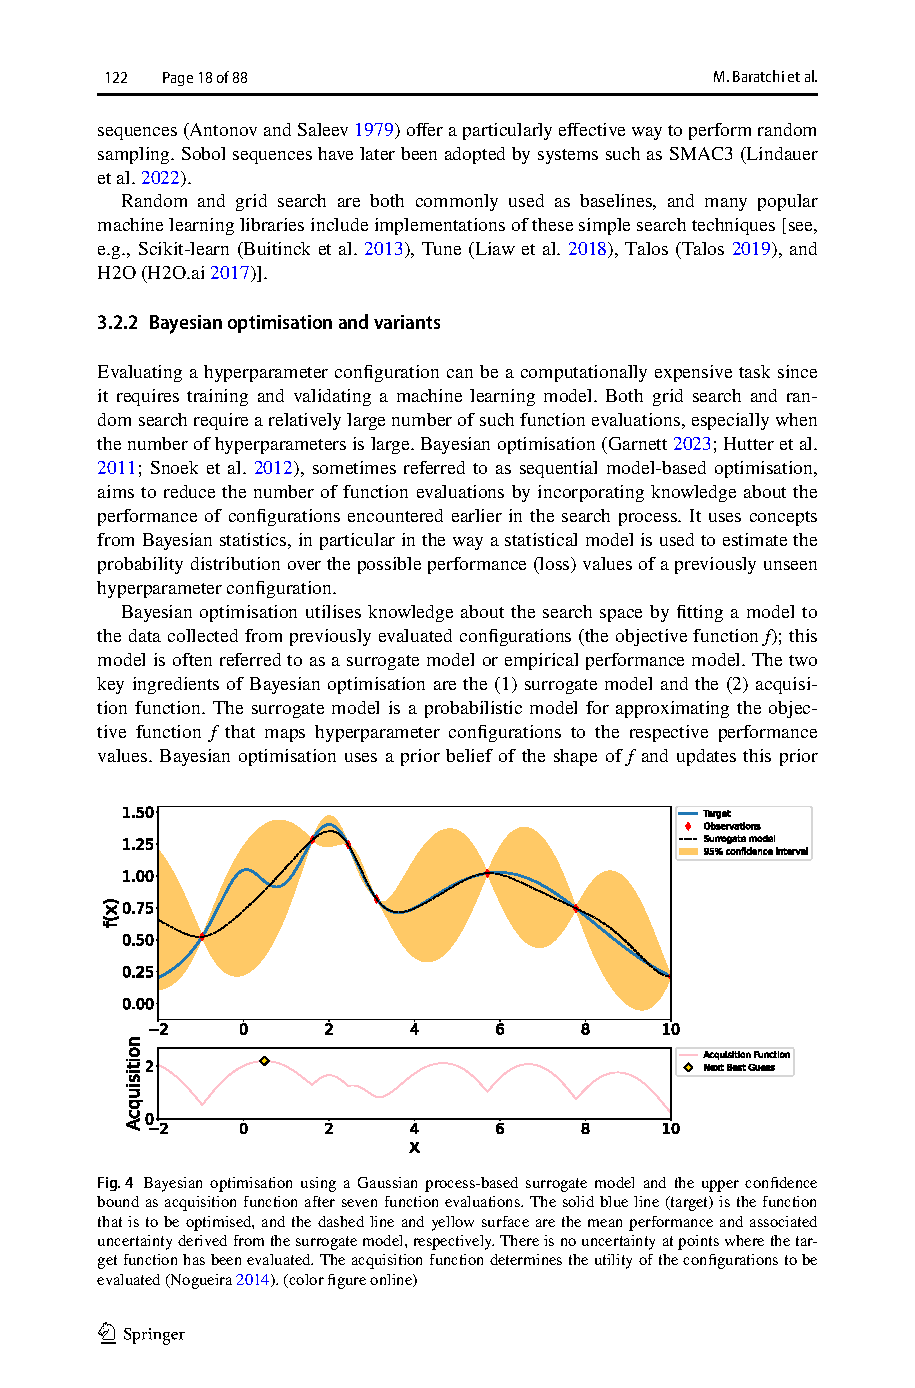
\includegraphics[width=0.8\linewidth,trim={2cm 4cm 2cm 13.5cm}, clip]{figures/985693BO.pdf}
    \caption{BO using a surrogate model and EI after several evaluations. The solid line represents the true objective $\mathcal{L}$, while the dashed line and shaded region show the surrogate mean and 95\% confidence interval, respectively. The acquisition function (bottom) determines the next candidate configuration to evaluate. \cite{AutoMLHoos}}
    \label{fig:bo_illustration}
\end{figure}

%Common algorithms used as surrogate models include \emph{Gaussian Processes} and \emph{Random Forests}. While Gaussian Processes provide good uncertainty estimates for continuous parameters, Random Forests are often preferred in \ac{AutoML} frameworks such as \ac{SMAC}, because they scale more efficiently and natively handle discrete and categorical hyperparameters \parencite{AutoMLHoos}. \me{maybe delete paragraph, irrelevant. also maybe dont explain Ei if i dont use it, but i think its fine as a baseline}


\subsubsection{Tree-structured Parzen Estimator} 

Rather than directly modeling the probability $p(y \mid \lambda)$ of observations $y$ given hyperparameter configurations $\lambda$, the \ac{TPE} \parencite{bergstra2011algorithms} instead constructs two separate density functions, $p(\lambda \mid y < \alpha)$ and $p(\lambda \mid y \geq \alpha)$. The threshold $\alpha$ partitions all observations into a set of good and bad configurations, each of which is modeled using one-dimensional Parzen windows. 
Parzen windows are kernel density estimators that place a smooth Gaussian function at each data point, with their sum forming the density function.
 The ratio $\frac{p(\lambda\mid y \ge \alpha)}{p(\lambda\mid y < \alpha)}$ is closely related to the expected improvement acquisition function and serves as the criterion for proposing new hyperparameter configurations \parencite{bergstra2011algorithms, hutter2019automated}. \ac{TPE} further scales linearly with the number of hyperparameters \parencite{AutoMLHoos}. %Through maintaining a sorted list of confgurations in memory, 





Search strategies are frequently paired with pruning mechanisms. Pruning, or early stopping, terminates the training of unpromising configurations before they consume their maximum allocated budget. Methods such as Successive Halving evaluate a large number of configurations for a few epochs, discard the worst-performing candidates and allocate more computational resources to the top performers.


\subsection{Performance evaluation}
To guide the search strategy, the \ac{AutoML} system must continuously evaluate the performance of each sampled configuration. The evaluation metric serves as the feedback signal for the search algorithm. It is critical to avoid overfitting to the validation data. If the search space is heavily optimized against a single validation set, the resulting hyperparameter configuration may fail to generalize to unseen test data \parencite{hutter2019automated}. Thus, robust evaluation protocols are necessary during the search phase to ensure the final model maintains its predictive accuracy in real-world deployment.


